
\chapter{基于SVR+Q的分块逼近模型在直复营销中的研究}

\section{研究动机}
直复营销是一个序贯决策过程,即随着时间的推移,营销人员需要不断的做出营销决策。所以,在进行决策时,营销人员不仅需要考虑到每个决策行为的成本和其收益之间的关系,而且还要考虑到营销序列上不同决策点之间的相互影响。

考虑如下场景:在某次营销决策时,营销人员发现如果对某一位客户进行营销,其产生的估计收益会大于营销成本,那么此时就不会对这位客户进行营销。但是,应该意识到即使此时该客户没有产生利润,但是这次的营销可能会增加该客户在以后的营销活动的中产生的利润,甚至该利润会很大。所以,营销人员在进行决策时,有时需要牺牲即时收益以获得长期收益最大化。反之亦然,如果频繁的对某一位高质量用户发送营销信息,会降低该客户所能产生的期望收益,因为每一位客户在一段时间内消费能力是固定的。

而传统的经典分类算法和基于代价敏感的改进分类算法,都只考虑到最大化单个独立决策事件的收益,并不能保证在一段时间上的长期收益最大化。考虑到强化学习是以累积收益最大化为目标,并且基于序列中的延迟影响来进行决策的学习,通过这种方式可以很好的处理序列决策中相互影响,进而达到长期收益最大化的目标,所以文献\citep{,pednault2002sequential,archak2010budget,boutilier2016budget}等提出使用强化学习的思想来解决直复营销问题。但是,在上述相关工作中,以下问题仍然没有得到解决:各营销决策点之间存在可变时间间隔会给奖赏数据带来一定的噪声影响,而且,随着数据规模的不断提升,值函数的收敛速度和学习速度都会变慢。

本文针对两个问题进行分析,本章提出了基于SVR+Q的分块逼近模型,用于更好的解决直效营销问题。首先,利用马尔科夫决策过程,将直复营销问题建模为一个强化学习问题;然后,为了解决决策点间的可变时间间隔问题,提出了改进的Q值函数更新方法;接着,为了高效的利用离线样本,结合Q-learning的学习方式,提出一种采样方法;最后,使用基于SVR+Q的分块逼近模型来逼近Q值函数,以加快值函数的收敛速度和逼近精度。

\section{基于SVR+Q的分块逼近模型}


\subsection{问题建模}
在第二章中提到,强化学习问题可以使用一个马尔可夫决策过程来描述:在任意给定的时间点上,假设环境处于某个状态,当Agent采取一个行为时,它会收到一个有限的奖赏,并且环境会相应的转移到下一个状态中。Agent选择的行为的依据是可以最大化累计奖赏,该奖赏通常是以累计折扣的形式表示。

对应到直复营销场景中,客户的状态可以使用客户在某一时刻所具有的特征信息来表示,比如文献\citep{tkachenko2015autonomous}中提到的Recency-Frequency-Monetary(最近交易时间、交易频率和交易金额)等,营销人员所采取的营销行为可以表示为Agent的行为,客户在营销反馈中所产生的价值作为奖赏信息。

在某一时刻,某一位客户历史的营销和消费信息,可以用来表示该客户此时的状态,如果营销人员对其采取了营销行为,那么该顾客的状态会发生改变,根据一定的转移概率转移到下一状态,并且在这一过程客户可能会产生一定的奖赏信息。以上这个过程始终贯穿于客户和营销人员的交互关系之中。需要注意的是,在客户状态发生转移时,所产生的奖赏信息是指该客户产生的消费金额减去相关成本后的净利润,如果客户没有发生消费购买行为,那么此时的奖赏值为负。也就是说,强化学习应用到该场景的任务就是最大化客户生命周期的净利润值。

本文考虑采用Q-learning(算法:$\ref{algo:algorithm_2}$)的强化学习方法作为框架,来解决以上问题。所以,可以使用$\{<S_{t},A_{t},R_{t}>\}_{t=1}^{\infty}$三元组来表示营销人员的每一次的营销事件。其中,$S_{t}$表示用户的状态,$A_{t}$表示营销人员所采取的行为,$R_{t}$表示此次营销所带来的奖赏。

\subsection{SVR+Q的分块逼近模型}
在传统的Q-learning算法中,值函数其实是一个表格,其索引是状态或者状态行为对,值迭代更新实际上就是这张表格的迭代更新。所以,Q-learning算法存在一个假设是,问题的状态空间和行为空间不能太大。然而,在像直复营销这类现实问题中,为了合理准确的表示客户的状态信息,需要非常多的特征进行表示,其状态空间自然非常大,所以,这时使用表格的形式进行表示并不现实。

如第二章所述,对于值函数的评估可以通过函数逼近的方法进行解决。在文献\citep{pednault2002sequential,archak2010budget,boutilier2016budget}中,针对值函数的逼近学习,作者了采用参数化线性函数逼近的方法。但是,参数化非线性函数逼近的方法常常会因为线性方法表达能力差而很难取得理想的逼近效果。考虑到基于非参数函数逼近方法的灵活性,并且可以充分利用样本进行训练,所以在本模型中,通过采用基于核函数的支持向量回归(Support Vector Regression, SVR)逼近模型,可以将值函数逼近问题转化为高纬特征空间的线性回归问题,在保证泛化能力的前提先有效提高算法的收敛速度。同时,结合针对离散行为的分块逼近思想,提升模型的逼近精度。

\paragraph{分块逼近思想}
考虑具有连续状态空间$S=\{S_{t}|t\in \mathbb{R}\}$和离散行为空间$A=\{A_{t}\}_{t=1}^{N}$的强化学习问题,可以将离散行为根据行为值的不同划分为$N$块,然后利用逼近模型M对该问题的Q值函数进行建模。$M=\{M_{i},\cdots,M_{N}\}$,其中$N$为划分的块数,每一块对应一类离散行为的数据样本集合,每个样本集合对应一个子模型,各子模型之间相互独立。

子模型可以采用任意的结构模型,若$N$个子模型结构相同,则称M为同构分块逼近模型,否则称为异构分块逼近模型。

\paragraph{SVR+Q逼近过程}
基于以上分块逼近的思想,本节利用SVR核函数的方法构建一组同构的逼近模型,来逼近Q值函数。下面详细介绍该模型的构建和逼近过程。

假设当前第$i$个行为对应的样本集合为$D_{i}=\{<\bm{X}_{ij}, Q_{ij}>\}_{j=1}^{N_{i}} \subseteq (\bm{S} \times A \times Y)^{N_{i}}$,其中$\bm{X}_{ij}=(\bm{S}_{ij}, A_{ij})$为样本$j$的输入向量,$Q_{ij}$为样本$j$的Q输出值,$N_{i}$为第$i$个渠道的样本数量,$(\bm{S} \times A) = \mathbb{R}^{n+1}$表示输入域,$Y \subseteq \mathbb{R}$表示输出域。

利用SVR+Q模型对值函数进行逼近时,以结构化风险最小为目标,学习一组仿射函数$\{f_{i}:(\bm{S} \times A) \mapsto Y\}$,$i=1,\cdots,I$。形式为:
\begin{equation}\label{seq:obj1}
\begin{aligned}
Q_{i}=f_{i}(\bm{s,a})=f_{i}(\bm{x})=\bm{w}_{i}^{T} \bm{\phi}(\bm{x}) + b_{i}, \quad i=1,2,\cdots,I
\end{aligned}
\end{equation}

式\eqref{seq:obj1}中,$\bm{\phi}(\cdot)$表示可以将样本从非线性空间映射到高维线性空间的函数,$\bm{w}_{i}$表示线性回归函数的权值向量,$b_{i}$是一个偏置项,$Q_{i}$是向量$\bm{x}$在第$i$个模型的Q输出值。根据SVR的原理,可以将原问题转化为带约束条件的优化问题:

\begin{equation}\label{seq:svr_ori}
\begin{split}
& \min_{\bm{w}_{i}, b_{i},\xi_{i}, \hat{\xi}_{i}}  J(\bm{w}_{i},b_{i},\xi_{i},\hat{\xi}_{i}) = \frac{1}{2} \left \| \bm{w}_{i} \right \|^{2} + C_{i} \sum_{j=1}^{N_{i}}(\xi_{ij}+\hat{\xi}_{ij})\\ 
& s.t. \begin{matrix}
& f_{i}(\bm{X}_{ij}) - Q_{ij} \leqslant \epsilon + \xi_{ij}\\
&Q_{ij} - f_{i}(\bm{X}_{ij})  \leqslant \epsilon + \hat{\xi}_{ij} \\
&\xi_{ij} \geqslant 0, \quad \hat{\xi}_{ij} \geqslant 0\\
& i=1,2,\cdots,I \quad j=1,\cdots,N_{i}
\end{matrix}
\end{split}
\end{equation}

式\eqref{seq:svr_ori}中,$\xi_{ij}$,$\hat{\xi}_{ij}$为松弛因子,$C_{i}$是正则化参数,用于控制对超出误差允许范围的样本的惩罚程度,$\bm{w}_{i}$为权值向量,用于控制模型的复杂程度。

引入拉格朗日乘子$\alpha_{ij} \geqslant 0$,$\hat{\alpha_{ij}} \geqslant 0$,$\mu_{ij} \geqslant 0$,$\hat{\mu_{ij}} \geqslant 0$,将原空间的约束优化问题转化为对偶空间的无约束优化问题,得到拉格朗日函数:

\begin{equation}\label{seq_lagrange}
\begin{aligned}
L_{i}(\bm{w}_{i}, b_{i}, \bm{\alpha}_{i}, \bm{\hat{\alpha}}_{i}, \bm{\xi}_{i}, \bm{\hat{\xi}}_{i},
\bm{\mu}_{i},\bm{\hat{\mu}}_{i})&=\frac{1}{2} \left \| \bm{{w}}_{i} \right \|^{2} + C_{i} \sum_{j=1}^{N_{i}}(\xi_{ij} + \hat{\xi}_{ij}) - \sum_{j=1}^{N_{i}}\mu_{ij}\xi_{ij} - \sum_{j=1}^{N_{i}}\hat{\mu}_{ij}\hat{\xi}_{ij} \\ 
&+ \sum_{j=1}^{N_{i}} \alpha_{ij}(\bm{w}_{i}^{T} \bm{\phi}(\bm{X}_{ij}) + b_{i} - Q_{ij} - \epsilon - \xi_{ij}) \\
&+ \sum_{j=1}^{N_{i}} \hat{\alpha}_{ij}(Q_{ij} - \bm{w}_{i}^{T} \bm{\phi}(\bm{X}_{ij}) - b_{i} - \epsilon - \hat{\xi_{ij}})\\
\end{aligned}
\end{equation}

对式$\eqref{seq_lagrange}$求偏导:
\begin{equation}\label{seq_lag_deri}
\begin{split}
&\frac{\partial{L_{i}}}{\partial{\bm{w}_{i}}}=0 \Rightarrow \bm{w}_{i} = \sum_{j=1}^{N_{i}}(\hat{\alpha}_{ij}-\alpha_{ij})(\bm{X}_{ij})
\\ 
&\frac{\partial{L_{i}}}{\partial{b_{i}}}=0 \Rightarrow 0 = \sum_{j=1}^{N_{i}}(\hat{\alpha}_{ij}-\alpha_{ij})
\\ 
&\frac{\partial{L_{i}}}{\partial{\xi_{ij}}}=0 \Rightarrow  C_{i} = \alpha_{ij} + \mu_{ij}
\\ 
&\frac{\partial{L_{i}}}{\partial{\hat{\xi}_{ij}}}=0 \Rightarrow  C_{i} = \hat{\alpha_{ij}} + \hat{\mu_{ij}}
\\
\end{split}
\end{equation}

将式\eqref{seq_lag_deri}求导结果代入式\eqref{seq_lagrange},即可得到SVR的对偶问题:

\begin{equation}\label{seq_lagr_dual}
\begin{split}
&\max_{\bm{\alpha}_{i}, \bm{\hat{\alpha}}_{i}} \sum_{j=1}^{N_{i}} Q_{ij}(\hat{\alpha}_{ij} - \alpha_{ij}) - \epsilon (\hat{\alpha}_{ij} + \alpha_{ij}) - \frac{1}{2} \sum_{j=1}^{N_{i}} \sum_{k=1}^{N_{i}}(\hat{\alpha_{ij}}-\alpha_{ij})(\hat{\alpha}_{ij}-\alpha_{ij})\bm{X}_{ij}^{T}\bm{X}_{ij},\\
&s.t. \sum_{j=1}^{N_{i}}(\hat{\alpha}_{ij}-\alpha_{ij})=0, \quad 0 \leqslant \alpha_{ij},\hat{\alpha}_{ij} \leqslant C.
\end{split}
\end{equation}

上述过程满足KKT(Karush-Kuhn-Tucker)最优化条件,即需要:
\begin{equation}
\label{seq_kkt}
\left\{\begin{matrix}
&\alpha_{ij}(\bm{w}_{i}^{T} \bm{\phi}(\bm{X}_{ij}) + b_{i} - Q_{ij} - \epsilon - \xi_{ij})=0
\\ 
&\hat{\alpha}_{ij}(Q_{i} - \bm{w}_{i}^{T} \bm{\phi}(\bm{X}_{ij}) - b_{i} - \epsilon - \hat{\xi}_{ij})=0
\\ 
&\alpha_{ij}\hat{\alpha}_{ij}=0, \xi_{ij}\hat{\xi}_{ij}=0
\\ 
&(C_{i}-\alpha_{ij})\xi_{ij}=0,\quad (C_{i}-\hat{\alpha}_{ij})\hat{\xi_{ij}}=0,
\\
\end{matrix}\right.
\end{equation}

将上述结果,可得SVR的解为:
\begin{equation}
\label{seq_svr_final}
f_{i}(\bm{x})=\sum_{j=1}^{N_{i}}(\hat{\alpha}_{ij}-\alpha_{ij})\bm{X}_{ij}^{T}\bm{X}+b_{i}
\end{equation}

在求解$\bm{X}_{ij}^{T}\bm{X}$这个内积的时候,如果输入样本线性不可分,我们可以通过$\bm{\phi}(\cdot):X \to F$函数映射,将输入样本映射到另外一个高维空间并使其线性可分。通常会选择满足Mercer定理的核函数$\bm{k}(\cdot,\cdot)$。目前应用较多的核函数有线性核函数、多项式核函数、RBF以及Sigmoid核函数等,考虑到RBF核函数简单性、计算难度小、算法易于实现等优点,故在本模型中采用RBF核函数,将优化问题表示为关于核函数的线性问题。
\begin{equation}
\bm{k}(\bm{x}_{a} - \bm{x}_{b}) = \exp{\frac{-\left \| \bm{x}_{a} - \bm{x}_{b} \right \|^{2}}{2\sigma^{2}}}
\end{equation}

所以,式$\eqref{seq_svr_final}$可化为:
\begin{equation}\label{seq_final}
\begin{aligned}
\text{Q}_{i}=f_{i}(\bm{x})=f_{i}(\bm{s},a)&=\bm{w}_{i}^{T} \bm{\phi}(s,a) + b_{i}\\
&=\sum_{j=1}^{N_{i}}(\hat{\alpha}_{ij}-\alpha_{ij})\bm{k}((\bm{s},a),(\bm{S}_{ij},A_{ij}))+b_{i}
\end{aligned}
\end{equation}

以上就是利用SVR+Q算法对第$i$个子模型进行Q值函数逼近的方法,在所有子模型都采用以上方法进行逼近后,再多路逼近Q值函数。

\paragraph{SVR+Q分块逼近模型更新}
在传统的Q-learning算法中,还存在另一个假设,就是Agent可以与环境进行在线的互动。然而,像在直复营销这类实际应用中,构建这样的在线交互环境在很难的。为了解决这个问题,通常采用批强化学习(Batch Reinforcement Learning)的方法进行解决\citep{lange2012batch},批强化学习是强化学习的一种形式,即Agent采取的行为、环境发生的状态转移都不以在线的方式进行,而是使用代表先前的经验的大量静态训练数据进行离线的学习。训练数据由状态向量、动作值以及奖赏值所组成的三元组来构成。这种批学习的方式反映了实际应用的真实交互情况。

在第二章中,我们知道强化学习值迭代的过程可表示为式$\eqref{seq_value_inter}$的形式:
\begin{equation}\label{seq_value_inter}
\begin{aligned}
&Q^{(0)}(s,a) = R(s,a) \\
&Q^{(p+1)}(s,a) = R(s,a) + \gamma \sum_{s^{'}} p(s^{'}|s,a) \max_{a^{'}} Q^{(p)}(s^{'},a^{'})
\end{aligned}
\end{equation}

其中,$R(s,a)$是指期望的即刻奖赏,$p(s^{'}|s,a)$表示在状态$s$下,采取行为$a$后,环境转移到下一状态$s^{'}$的概率。

所以,给定好训练数据,以及模型的逼近方法后,参考上式$\eqref{seq_value_inter}$值迭代的更新方法,就可以进行Q值的估计了。具体地,在第一次的迭代过程中,使用逼近模型SVR+Q来预测基于状态s和行为a的期望即刻奖赏值$R(s,a)$,在第二次以及之后的迭代过程中,再次使用上述逼近模型SVR+Q,依据Q值函数的更新公式$\eqref{seq_value_q}$进行更新,以得到改进的Q值函数。
\begin{equation}\label{seq_value_q}
\begin{aligned}
Q(S_{t}, A_{t}) \gets Q(S_{t}, A_{t}) + \alpha (r_{t+1} + \gamma \max_{a} Q(S_{t}, a) - Q(S_{t}, A_{t}))
\end{aligned}
\end{equation}

结合以上批强化学习方法和基于SVR+Q的分块逼近模型,图$\ref{algo:SVR+Q}$给出了基于SVR+Q模型伪代码。

\begin{algorithm}[htbp]
\small
\SetAlgoLined
\SetKwRepeat{Repeat}{repeat}{until} 
\KwData{折扣因子$\gamma$,正则化参数$C$,RBF核函数的宽度$\sigma$,最大迭代次数$P$,原始样本$D=\{e_{i}|i=1,\cdots,I\}$,$e_{i}=\{<S_{i,j}, A_{i,j}, R_{i,j}>|j=1,\cdots,l_{i}\}$,($D$表示样本集合,$e_{i}$表示第$j$个情节,$l_{i}$表示$e_{i}$的长度)}
\KwResult{输出最终的逼近模型:$Q^{(P)}$}

\For{all $e_{i} \in D$}{
	初始化第$i$个情节的数据:$D_{i}^{(0)}=\{<S_{i,j}, A_{i,j}, R_{i,j}>|j=1,\cdots,l_{i}\}$\;
}
整合所有情节的数据,生成总样本集合:$D^{(0)}=\cup_{i=1,\cdots,I} D_{i}^{(0)}$\;
将总样本集合$D^{(0)}$,按照行为标签ID$(A_{i,j}) \in \{1,2,\cdots, K \}$分发到各子模型的样本集合中,并利用SVR+Q模型的公式$\eqref{seq_final}$分别逼近值函数:$Q_{k}^{(0)}$, $k=1,\cdots,K$\;
多路逼近Q值函数:$Q^{(0)}=\cup_{k=1,\cdots,K},Q_{k}^{(0)}$\;
\For{$p=1$ \KwTo $P$}{
	\For{all $e_{i} \in D$}{
		\For{$j$ \KwTo $l_{i}-1$}{
			利用公式$\eqref{seq_value_q}$更新状态行为值:\;
			$v_{i,j}^{(p)}=Q^{(p-1)}(S_{i,j},A_{i,j}) + \alpha^{(p)} (R_{i,j} + \gamma \max_{a} Q^{(p-1)}(S_{i,j+1},a)-Q^{(p-1)}(S_{i,j},A_{i,j}))$\;
		}
		更新第$i$个情节的样本:$D_{i}^{(p)}=\{<S_{i,j}, A_{i,j}, v_{i,j}^{(p)}>|j=1,\cdots,l_{i}-1\}$\;
	}
	整合所有情节的数据,生成总样本集合。$D^{(p)}=\cup_{i=1,\cdots,I}D_{i}^{(p)}$\;
	将总样本集合$D^{(p)}$,按照行为标签ID$(A_{i,j}) \in \{1,2,\cdots, K \}$ 分发到各子模型的样本集合中,并利用SVR+Q模型的公式$\eqref{seq_final}$分别逼近值函数:$Q_{k}^{(p)}$,$k=1,\cdots,K$\;
	多路逼近Q值函数:$Q^{(p)}=\cup_{k=1,\cdots,K} Q_{i}^{(p)}$\;
}
\caption{SVR+Q算法}
\label{algo:SVR+Q}
\end{algorithm}

在伪代码$\ref{algo:SVR+Q}$中,按照批强化学习的训练方法,将训练数据集$D$(总样本集合)分成$I$个情节(episode),每个情节由一系列事件(event)组成,每个事件包含状态、行为和奖赏信息信息。在情节数据中,保持了事件原有的出现顺序,以此来重现真实的交互的过程。

在第一轮迭代中,首先要初始化每个情节中的数据,整合成总样本集合$D^{(0)}$,然后按照总样本集合中行为标签值的不同划分$K$子样本集合,然后利用SVR+Q模型中公式$\eqref{seq_final}$对即刻奖赏信号进行预测,以此作为初步的估计Q值函数。在第二轮及之后的迭代过程中,结合上一次的估计值函数,利用Q值函数的更新公式$\eqref{seq_value_q}$更新每个情节中每一个事件的状态行为值。当每一轮训练结束后,就将更新后的样本情节进行整合,形成总样本集合$D^{(p)}$,并按照行为标签值的不同划分$K$子样本集合,然后利用SVR+Q模型中公式$\eqref{seq_final}$逼近每个行为的Q值函数,再多路逼近Q值函数$Q^{(p)}$。当所有轮数迭代完毕后,输出最终的Q值函数。另外,对算法中学习率$\alpha_{i}$的选取,通常设置为$\alpha_{i}=\frac{1}{K}$,目的是让学习的步伐随着迭代次数的增加而不断减小。

\subsection{可变时间间隔问题}
在标准马尔科夫决策过程中,假设每个决策点之间的时间间隔是固定的,所以,如果假设在时刻$t$后接收到的奖赏序列为$\{R_{t+1}, R_{t+2},\cdots\}$,那么采用折扣累积奖赏的方式计算回报可用公式$\eqref{seq:reward_3}$来表示:
\begin{equation}\label{seq:reward_3}
G_{t}=\sum_{k=0}^{\infty}\gamma^{k}R_{t+k+1}
\end{equation}
式$\eqref{seq_final}$中,$G_{t}$为回报,$\gamma<1$,为一个常量,称为折扣因子。

但是,在直复营销过程中,各个营销决策点之间的时间间隔是不确定的,比如相邻的两个营销时间有的间隔时间长,有的间隔时间比较短,所以就存在可变时间间隔的问题。如果采用公式$\eqref{seq:reward_3}$的方式计算累积奖赏,会带来一定的噪声影响,所以就要改变算法$\ref{algo:SVR+Q}$中的更新方式,以减少这种噪声给值函数的估计带来的影响。
如图$\ref{fig:2_ad_process}$所示。
\begin{figure}[htbp]
\centering
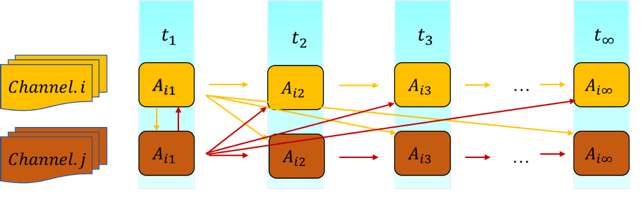
\includegraphics[width=0.8\textwidth]{2_ad_process}
\caption{广告在两个渠道上的生命周期}
\label{fig:2_ad_process}
\end{figure}

和标准的马尔科夫决策过程相比,在带有可变时间间隔的马尔科夫决策过程中,每次的交互事件都会被标记上时间。假设将初始状态的时刻记为$0$,那么后续交互事件被标记的时间都大于0。假设整个马尔科夫决策过程是从$t_{1}=0$时刻开始的,并且初始状态为$S_{1}$,之后agent重复的采取行为,便会得到一系列的由行为、状态、奖赏以及时间组成的四元组$\{<S_{i},A_{i},R_{i},t_{i}>\}_{i=1}^{\infty}$,其中$t_{i}$就是第$i$个时间发生的时间。那么,在计算累积折扣奖赏时,折扣因子就被定义为关于时间的函数,如式\eqref{seq:r}所示:
\begin{equation}\label{seq:r}
\begin{aligned}
G_{t}=\sum_{i=1}^{\infty} \gamma^{t_{i}}R_{i}
\end{aligned}
\end{equation}

在可变时间间隔的马尔科夫决策过程中,需要为可变长时间间隔中的奖赏找到一个合适的标准化方法,以减少可变时间间隔给奖赏的计算所带来的噪声。通常的做法是采用将一个时间间隔内收到的奖赏除以时间间隔长度的方式进行标准化。如\eqref{seq:r_1}所示:
\begin{equation}\label{seq:r_1}
\begin{aligned}
R_{i}^{'}=\frac{R_{i}}{t_{i+1}-t_{i}}=\frac{R_{i}}{\triangle t_{i}}
\end{aligned}
\end{equation}

在对原始奖赏值$R_{i}$进行标准化后,就要按照算法$\ref{algo:SVR+Q}$中第4行和第5行的方式进行更新样本,并利用样本得到奖赏的估计模型。那么,此时更新值函数的时候,第11行的更新公式就要按照如下式\eqref{seq:r_2}的方式进行更新:
\begin{equation}\label{seq:r_2}
\begin{aligned}
v_{i,j}^{(p)}=&(1-\alpha^{(p)})Q^{(p-1)}(S_{i,j},A_{i,j}) \cdot \triangle t_{i,j} \\
&+ \alpha^{(p)} (R_{i,j} + \gamma^{\triangle t_{i,j}} \max_{a} Q^{(p-1)}(S_{i,j+1,},a) \cdot \triangle t_{i,j+1})
\end{aligned}
\end{equation}

从式\eqref{seq:r_2}可以看到,时间间隔$\triangle t_{i,j}$在更新的时候,会受到学习率$\alpha^{(p)}$的影响。比如,随着学习率的的升高,时间间隔的值也在增加,就相当于给值函数的更新赋予更大的权重。所以,在更新Q值函数$v_{i,j}$的时候,还要考虑到对时间间隔的更新。

因为考虑到上述问题产生的原因主要是受学习率的影响,所以本文基于时间间隔构建一个标准化因子,并仿照Q值函数的更新方式进行标准化因子的更新,以解决之前更新方式所带来的偏差影响。设标准化因子为$Z_{i,j}$,那么其更新方式可表示为式\eqref{seq:r_3}
\begin{equation}\label{seq:r_3}
\begin{aligned}
Z^{(p)}_{i,j}=(1-\alpha^{(p)})Z^{(p-1)}_{i,j}+\alpha^{(p)}(\triangle t_{i,j} + \gamma^{\triangle t_{i,j}} \cdot Z^{(p-1)}_{i,j+1})\;
\end{aligned}
\end{equation}

由此,本节得到基于可变时间间隔的SVR+Q的算法如$\ref{algo:RBF-SVR-Q-t}$所示。其中,第1行到第5行进行时间间隔的计算,第6行到第12行进行标准化因子以及样本的的初始化,第18行进行Q值函数的更新,此处对应时刻点的Q值函数要乘以对应时刻点的归一化因子,第20行进行归一化因子的更新。

\subsection{改进的采样方法}
在直复营销等类似的应用场景中,产生的数据量非常大,如果将全部样本都导入逼近模型中进行训练,将必然会加重模型的训练负担,另外,Q值函数的更新也会消耗很多的时间。所以,为了解决以上问题,应该采取有效的采样方法来加快模型的训练和更新速度。
\begin{algorithm}[htbp]
\small
\SetAlgoLined
\SetKwRepeat{Repeat}{repeat}{until} 
\KwData{折扣因子$\gamma$,正则化参数$C$,RBF核函数的宽度$\sigma$,最大迭代次数$P$,原始样本$D=\{e_{i}|i=1,\cdots,I\}$,$e_{i}=\{<S_{i,j}, A_{i,j}, R_{i,j}, t_{i,j}>|j=1,\cdots,l_{i}\}$,($D_{i}$表示第$i$个渠道的样本,$e_{i,j}$表示第$i$个渠道第$j$个情节,$l_{i,j}$为$e_{i,j}$的长度)}

\KwResult{输出最终的逼近模型:$Q^{(P)}$}

\For{all $e_{i} \in D$}{
	\For{$j$ \KwTo $l_{i}$}{
		计算时间间隔,$\triangle t_{i,j}=t_{i,j+1}-t_{i,j}$\;
	}
}
\For{all $e_{i} \in D$}{
	\For{$j$ \KwTo $l_{i}-1$}{
		得到初始的标准化因子:$Z^{(0)}_{i,j}=\triangle t_{i,j}$\;
		得到初始的状态值:$v^{(0)}_{i,j} = R_{i,j}$\;
		将初始的状态值使用标准化因子进行标准化:$D_{i}^{(0)}=\{<S_{i,j}, A_{i,j}, \frac{v^{(0)}_{i,j}}{Z^{(0)}_{i,j}}>|j=1,\cdots,l_{i}\}$\;
	}
}

同算法$\ref{algo:SVR+Q}$中第4行到第6行\;
% 整合所有情节的数据,生成总样本集合:$D^{(0)}=\cup_{i=1,\cdots,I} D_{i}^{(0)}$\;
% 将总样本集合$D^{(0)}$,按照行为标签ID$(A_{i,j}) \in \{1,2,\cdots, K \}$分发到各子模型的样本集合中,并利用SVR+Q模型的公式$\eqref{seq_final}$分别逼近值函数:$Q_{k}^{(0)}$, $k=1,\cdots,K$\;
% 多路逼近Q值函数:$Q^{(0)}=\cup_{k=1,\cdots,K},Q_{k}^{(0)}$\;

\For{$p=1$ \KwTo $P$}{
	\For{all $e_{i} \in D$}{
		\For{$j$ \KwTo $l_{i}-1$}{
			更新Q值函数\;
			$v_{i,j}^{(p)}=(1-\alpha^{(p)})Q^{(p-1)}(S_{i,j},A_{i,j}) \cdot \triangle  Z_{i,j}^{(p-1)} 
			+ \alpha^{(p)} (R_{i,j} + \gamma^{\triangle t_{i,j}} \max_{a} Q^{(p-1)}(S_{i,j+1,},a) \cdot \triangle  Z_{i,j+1}^{(p-1)} )$\;
			更新标准化因子\;
			$Z^{(p)}_{i,j}=(1-\alpha^{(p)})Z^{(p-1)}_{i,j}+\alpha^{(p)}(\triangle t_{i,j} + \gamma^{\triangle t_{i,j}} \cdot Z^{(p-1)}_{i,j+1})$\;
			% 更新第$j$个情节的样本:$D_{i,j}^{(p)}=\{<S_{i,j,k}, A_{i,j,k}, \frac{v_{i,j,k}^{(p)}}{Z^{(p)_{i,j,k}}}>|k=1,\cdots,l_{i,j}-1\}$\;
		}
		更新第$i$个情节的样本:$D_{i}^{(p)}=\{<S_{i,j}, A_{i,j}, \frac{v_{i,j}^{(p)}}{Z^{(p)_{i,j}}}>|j=1,\cdots,l_{i}-1\}$\;
	}
	% 整合所有情节的数据,生成总样本集合。$D^{(p)}=\cup_{i=1,\cdots,I} D_{i}^{(p)}$\;
	% 将总样本集合$D^{(p)}$,按照行为标签ID$(A_{i,j}) \in \{1,2,\cdots, K \}$ 分发到各子模型的样本集合中,并利用SVR+Q模型的公式$\eqref{seq_final}$分别逼近值函数:$Q_{k}^{(p)}$,$k=1,\cdots,K$\;
	% 多路逼近Q值函数:$Q^{(p)}=\cup_{k=1,\cdots,K} Q_{i}^{(p)}$\;
	同算法$\ref{algo:SVR+Q}$中第15行到第17行\;
}
输出最终的逼近值函数$Q^{(P)} = Q^{(P)} \cdot Z^{(P)}$\;
\caption{基于可变时间间隔的SVR+Q算法}
\label{algo:RBF-SVR-Q-t}
\end{algorithm}

在强化学习中,通常的采样方法主要有随机采样法和Q-采样法,随机采样法,就是在每次从数据集中取情节的时候(如算法$\ref{algo:RBF-SVR-Q-t}$中,第6行和第15行),并不是取所有的情节,而是随机选取部分的情节,这种随机采样方法虽然可以减轻模型的训练和值函数的更新时间,但是采样后的数据质量并不高,因而会影响最后值函数的逼近效果。Q-采样法,在随机采样的基础上,当进行Q值函数的更新时,不是每个情节中所有事件都会被选择用于值函数的更新,而只有利用当前的估计Q值函数,可以在下一个状态中取得最佳行为的状态才能被选择。即在算法$\ref{algo:RBF-SVR-Q-t}$的第11到21行替换成如下算法$\ref{algo:SVR+Q_}$的语句:

\begin{algorithm}[htbp]
\small
\SetAlgoLined
\SetKwIF{If}{ElseIf}{Else}{if}{then}{else if}{else}{endif}
从数据集合$D$中随机采样一个样本子集,$R^{(p)}$\;
\For{all $e_{i} \in R^{(p)}$}{
	\For{$j$ \KwTo $l_{i}-1$}{
		\If{$Q^{(p-1)}(S_{i,j+1},A_{i,j+1})=\max_{a}Q^{(p-1)}(S_{i,j+1},a)$}{
			$v_{i,j}^{(p)}=(1-\alpha^{(p)})Q^{(p-1)}(S_{i,j},A_{i,j}) \cdot Z_{i,j}^{(p-1)} 
			+ \alpha^{(p)} (R_{i,j} + \gamma^{\triangle t_{i,j}} \max_{a} Q^{(p-1)}(S_{i,j+1,},a) \cdot  Z_{i,j+1}^{(p-1)} )$\;
			$Z^{(p)}_{i,j}=(1-\alpha^{(p)})Z^{(p-1)}_{i,j}+\alpha^{(p)}(\triangle t_{i,j} + \gamma^{\triangle t_{i,j}} \cdot Z^{(p-1)}_{i,j+1})$\;
		}
		更新第$i$个情节的样本:$D_{i}^{(p)}=D_{i}^{(p)} \cup \{<S_{i,j}, A_{i,j}, v_{i,j}^{(p)}>\}$\;
	}
}
\caption{基于Q采样的算法}
\label{algo:SVR+Q_}
\end{algorithm}

但是,通过Q采样的方法进行采样后的样本仍然很大,而且,即使选择了在下一状态中可以达到最佳行为的当前状态,但是该状态并不一定会有很高的学习效率。

考虑在本文第二章中,由公式$\eqref{shijiachafen}$计算出的$t$时刻的时间差分TD:$\delta_{t}$,应用在算法$\ref{algo:SVR+Q_}$的Q值函数中,可表示为式$\eqref{shijiachafenq}$:
\begin{equation}\label{shijiachafenq}
\begin{aligned}
&\delta_{i,j}=R_{i,j} + \gamma^{\triangle t_{i,j}} Q^{(p-1)}(S_{i,j+1}, a) \cdot Z_{i,j+1}^{(p-1)}  - Q^{(p-1)}(S_{i,j},A_{i,j}) \cdot Z_{i,j}^{(p-1)} \\
&\text{其中,} a=\argmax_{a} (Q^{(p-1)}(S_{i,j+1},a) \cdot Z_{i,j+1}^{(p-1)})
\end{aligned}
\end{equation}

式$\eqref{shijiachafenq}$中,$R_{i,j} + \gamma^{\triangle t_{i,j}} Q^{(p-1)}(S_{i,j+1}, a) \cdot Z_{i,j+1}^{(p-1)}$称为TD目标,即值函数逼近的目标值。如果TD偏差$\delta_{t}$越大,说明该状态处的值函数$Q^{(p-1)}(S_{i,j},A_{i,j}) \cdot Z_{i,j}^{(p-1)}$与TD目标目标的差距越大,进一步说明agent的更新量越大,因此在该处的学习效率就越高。所以,在抽样的时候,可以根据TD偏差的大小再一次进行有选择的采样。具体地,当使用Q采样算法$\ref{algo:SVR+Q_}$第4行条件进行初步选择后,设定一个固定的阈值$\eta$,然后使用公式$\eqref{shijiachafenq}$再一次进行选择,只选择TD偏差大于$\eta$的样本进行更新。所以,算法$\ref{algo:SVR+Q_}$可以修改为$\ref{algo:SVR+Q_2}$的形式。

\begin{algorithm}[htbp]
\small
\SetAlgoLined
\SetKwIF{If}{ElseIf}{Else}{if}{then}{else if}{else}{endif}
\KwData{增加一个TD偏差阈值$\eta$}
从数据集合$D$中随机采样一个样本子集,$R^{(p)}$\;
\For{all $e_{i} \in R_{k}$}{
	\For{$j$ \KwTo $l_{i}-1$}{
		\If{$Q^{(p-1)}(S_{i,j+1},A_{i,j+1})=\max_{a}Q^{(p-1)}(S_{i,j+1},a)$ $\bm{And}$
			利用公式$\eqref{shijiachafenq}$计算的$\delta_{i,j} \geqslant$  $\eta$
		}{
			$v_{i,j}^{(p)}=(1-\alpha^{(p)})Q^{(p-1)}(S_{i,j},A_{i,j}) \cdot Z_{i,j}^{(p-1)} 
			+ \alpha^{(p)} (R_{i,j} + \gamma^{\triangle t_{i,j}} \max_{a} Q^{(p-1)}(S_{i,j+1,},a) \cdot  Z_{i,j+1}^{(p-1)} )$\;
			$Z^{(p)}_{i,j}=(1-\alpha^{(p)})Z^{(p-1)}_{i,j}+\alpha^{(p)}(\triangle t_{i,j} + \gamma^{\triangle t_{i,j}} \cdot Z^{(p-1)}_{i,j+1})$\;
		}
		更新第$i$个情节的样本:$D_{i}^{(p)}=D_{i}^{(p)} \cup \{<S_{i,j}, A_{i,j}, v_{i,j}^{(p)}>\}$\;
	}
}
\caption{基于TD偏差的Q采样算法}
\label{algo:SVR+Q_2}
\end{algorithm}

\section{仿真实验}
本节,我们选择在直效营销中最经典的直邮营销场景中,研究第三章基于RNN的深度强化学习混合模型及其他的基准模型的应用效果。首先,对实验所使用的数据进行介绍,然后描述按照文献\citep{pednault2002sequential}中的方法构建仿真环境的过程,最后将模型的训练效果在仿真环境中进行测试评估,并且对测试结果进行分析。

\subsection{数据集}
\paragraph{数据集背景}
直邮营销是直效营销中最早的、也是最为经典的应用场景,它是通过对目标客户以邮寄营销信件的方式达到营销宣传的目的。本实验中选择使用UCI数据库中关于直邮营销著名的公开数据集KDD-CUP 1998\footnote{https://kdd.ics.uci.edu/databases/kddcup98/kddcup98.html}作为训练数据,并以此数据集构建仿真环境。需要提到的是,一些关于强化学习技术在直邮营销的研究文献\citep{pednault2002sequential,tkachenko2015autonomous}也都使用了该数据集。

KDD-CUP 1998数据集是由美国非盈利组织PVA(Paralyzed Veterans of America)收集的,该组织通过直邮的方式向潜在捐助者发布捐助活动信息以
筹集资金,为有脊髓损伤疾病的美国退伍军人提供援助。所以,该数据集是由在直邮捐助活动过程中所产生的信息组成,这些信息主要包括个人的基本信息以及两年所进行的23次募捐活动的历史反馈纪录,比如,该是否向该捐助者进行了邮寄、该捐助者是否产生捐助、产生了多少捐助金额等,另外邮寄的时间以及捐助者的回复时间都是可获得的。训练集中包括95412名捐助者在23个捐助活动过程中超过200万次的捐助反馈信息,其中23个捐助活动中又含有11种不同类型的邮件。有关数据集的其它描述信息可在UCI网站上获得。

\paragraph{数据结构}
我们的目标是要为下一个捐助活动提供直邮对象的名单,以及确定应该选择哪一种邮件类型,以使得PVA可获得的累积捐赠额最大化。所以,在KDD-CUP 1998数据集中,我们可供选择的行为有12个,包括11中不同的邮件类型以及一个不发送邮件的行为。因为数据集中包括23个不同时间段的捐助活动,所以,每一个捐助者的捐助历史纪录都可以看作是一个含有23个步骤的时间序列。因此,我们可以用如下长度为67(3*22+1)的序列表示一个捐助者的信息:($o_{1}, a_{1}, r_{1},\cdots,o_{22}, a_{22}, r_{22}, o_{23}$)。其中:

(1)$o_{t}$:捐助者在$t$时刻的可观测信息。主要内容如表~\ref{tab:obser_donors}所示。从表中可以看到,除了age和income特征信息可以直接从数据库中获得以外,其余的可观测特征都可以经过简单的统计运算获得。另外,需要注意的是,后面三个观测特征是基于一个时间周期为六个月的历史窗口总结得到的。所以,在提取特征时,每一条序列数据中前六个月的直邮募捐数据将作为第一个历史窗口,因此,序列数据的长度就变成了49:($o_{1}, a_{1}, r_{1},\cdots,o_{16}, a_{16}, r_{16}, o_{17}$)。
\begin{table}[htbp]
  \centering
  \caption{捐助者的可观测特征}
  \label{tab:obser_donors}
  \begin{tabular}{cl}
    \toprule
      可观察特征 & 描述 \\
    \midrule
      age & 捐助者的年龄 \\
      income & 捐助者的收入 \\
      dontimes & 捐助者捐助的次数 \\
      protimes & 向捐助者邮寄的次数 \\
      frequency & 捐助者捐助的频率:dontimes/protimes\\
      recency & 最近一次捐助距离此时的时间(月) \\
      monetary & 平均的捐助额 \\
      protimes_6 & 最近六个月里该捐助者收到募捐邮件次数 \\
      dontimes_6 & 最近六个月里该捐助者募捐的次数 \\
      montimes_6 & 最近六个月里该捐助者募捐的金额 \\
    \bottomrule
  \end{tabular}
\end{table}

(2)$a_{t}$:上述中提到PVA可采取的12个行为。$\{0,1,2,\cdots,11\}$其中,数字$0$表示不邮寄,其余$1$到$11$数字分别对应一种邮件类型。

(3)$r_{t}$:在执行行为$a_{t}$所能得到的即刻奖赏,对应到数据库中就是捐助者所捐助的金额数减去每条邮寄的成本。

\subsection{仿真环境}
在强化学习中,测试、评价模型的好坏需要有稳定的仿真环境。目前,openai提供了许多游戏的仿真环境开源库,科研人员可以通过其提供api接口非常方便的调用这些仿真器,来训练、测试自己模型,所以,这也是目前大多数强化学习的研究者选择在游戏领域进行研究的一个重要方面。然而,在其它的一些应用中,需要研究人员自己根据训练数据构建仿真器。本文中,针对直邮募捐活动,我们按照文献\citep{pednault2002sequential}提供的方法,通过构建关于训练数据集的马尔科夫决策过程对来搭建仿真器,进而评价模型的好坏。

构建的马尔科夫决策过程主要有两个评估模型组成:第一个模型$P(s,a)$是用来预测捐助者的产生反馈的概率,它是一个关于状态特征和行为的函数。第二个模型$A(s,a)$用来预测如果当募捐着对此次募捐邮件产生了反馈,会产生多少募捐额。其中,模型$P(s,a)$使用了基于朴素贝叶斯的树算法进行构建,模型$A(s,a)$使用线性回归树算法尽心构建。

当有了模型$P(s,a)$和$A(s,a)$,我们可以使用如下过程来构建马尔科夫决策过程。

1)给定状态$s$和行为$a$下的即时奖赏$r(s,a)$可以通过这两个模型得到:以$P(s,a)$的概率来掷一枚硬币,并以此来判断捐助者是否会产生反馈。即:出现正面的概率为$P(s,a)$表示捐助者会产生反馈,出现反面的概率为$1-P(s,a)$表示捐助者忽略掉了本次募捐邮件,没有产生任何反馈信息。如果没有出现反馈,那么捐助额为$0$,如果产生了反馈,那么用户的捐助金额为$A(s,a)$。即时奖赏$r(s,a)$等于捐助额减去邮寄的成本。

2)状态转移方程也可以通过使用这两个模型计算每一个观测状态的转移而得到。比如:如果以上述方式掷硬币出现正面朝上,那么观测值dontimes(捐助者捐助的次数)将会加$1$,否则,其值不发生变化。同样的,如果行为$1$到$11$任意一个值出现,那么观测值protimes(向捐助者邮寄的次数)会加$1$,如果行为$0$出现,那么其值保持不变。有了以上这两个值,观测值frequency就可以通过(dontimes/protimes)的方式得到。其它特征也可以通过这种方式更新得到。

有了上述马尔科夫决策过程的公式化定义,我们就可以使用如下的方式来构建我们的评估实验。1)首先选择一定数量规模(10000)的捐助者,并设置他们的初始状态,本实验中将所选择的捐助者的初始状态设置为第23个邮寄活动的状态,即$o_{23}$。2)然后使用强化学习模型的Q值函数来决定对每个捐献者应该采取哪一个行为。3)使用模型$P(s,a)$和$A(s,a)$,我们可以得到预估的即时奖赏以及下一时刻的状态。记录这些得到信息,然后进入下一次的邮寄决策中。就这样,按照上述的过程,每进行一次就会模拟一次虚拟的直邮募捐的过程。

在文献\citep{pednault2002sequential}中作者提出,构建上述仿真环境的假设前提是认为募捐者的交互过程是一个马尔科夫决策过程,然而这不一定是合适的。但是,将模型的环境构建为一个马尔科夫决策过程,然后使用一个强化学习算法从交互中去评价状态行为值函数是一个普遍采用的做法。作者认为,像直复营销这种与人类行为有关的场景都过于复杂,使用简单的MDP是无法较好的捕捉到环境的变化规律的,我们使用这个模拟器去评估我们的算法所产生的策略,只是在真实场景应用前的一个评估实验。所以,这种评估方法是可接受的,也是目前强化学习评估实验所普遍采用的方法。

\subsection{仿真结果}

\paragraph{生命周期价值}

\paragraph{直邮的数量}

\paragraph{每次直邮募捐的利润}

\paragraph{不同数据规模的效果比较}

\section{本章小结}
